\documentclass[a4paper,12pt]{article}

%% Language and font encodings
\usepackage[T1]{fontenc}
\usepackage[polish]{babel}
\usepackage[utf8]{inputenc}
\usepackage{lmodern}
\selectlanguage{polish}

%% Sets page size and margins
%\usepackage[a4paper,top=2cm,bottom=2cm,left=2cm,right=4cm,asymmetric]{geometry}
\usepackage{geometry}


%% Useful packages
\usepackage[fleqn]{amsmath}%[fleqn]
\usepackage{xfrac} %\sfrac{}{}

\usepackage{titlesec}%titles
\titlelabel{\thetitle.\quad}
\let\savenumberline\numberline
\def\numberline#1{\savenumberline{#1.}}
\usepackage{etoolbox}%dots in TOC
\makeatletter
\patchcmd{\l@section}
{\hfil}
{\leaders\hbox{\normalfont$\m@th\mkern \@dotsep mu\hbox{.}\mkern \@dotsep mu$}\hfill}
{}{}
\makeatother

\usepackage{caption,graphicx}
\usepackage{float}
\usepackage{sidecap}
\usepackage[colorinlistoftodos]{todonotes}
\usepackage[colorlinks=true, allcolors=blue]{hyperref}

\usepackage{tikz}
\usepackage{tikz-qtree}
\usetikzlibrary{trees}
\usetikzlibrary{arrows,positioning,shapes,fit,calc,decorations.pathreplacing}
\usetikzlibrary{graphs}
\usetikzlibrary{graphs.standard}
\usepackage{forest}
\usepackage{tikzscale}
\usepackage{pgfgantt} %Diagramy gantta http://bay.uchicago.edu/CTAN/graphics/pgf/contrib/pgfgantt/pgfgantt.pdf
\usepackage{pgf}
\usepackage{caption}

\usepackage{fancybox}
\usepackage{listings}

\usepackage[colorinlistoftodos]{todonotes} %http://mirror.unl.edu/ctan/macros/latex/contrib/todonotes/todonotes.pdf

\usepackage{array,longtable}

\newcommand\floor[1]{\lfloor#1\rfloor} %PODŁOGA -> \floor
\newcommand\ceil[1]{\lceil#1\rceil} %SUFIT -> \ceil

\usepackage{fancyhdr}
\pagestyle{fancy}
\rhead{\thepage}
\lhead{\leftmark}
\rfoot{\thepage}
\lfoot{\rightmark}

%http://tex.stackexchange.com/questions/64170/which-package-to-use-for-writing-algorithms
\usepackage{algorithm}% http://ctan.org/pkg/algorithms
\usepackage{algpseudocode}% http://ctan.org/pkg/algorithmicx
\newcommand{\var}[1]{{\ttfamily#1}}% variable

\algnewcommand\algorithmicforeach{\textbf{for each}} %Algorithm foreach
\algdef{S}[FOR]{ForEach}[1]{\algorithmicforeach\ #1\ \algorithmicdo}

\usepackage{amsthm}
\usepackage[inline]{enumitem} %enumerations
\usepackage{multicol}

\theoremstyle{definition}%~ %%% <-  Note that space!
\newtheorem{lemma}{Lemat} %\begin{lemma} ... \end{lemma} LEMAT(?)
\newtheorem{remark}{Wniosek}%\begin{remark} ... \end{remark} WNIOSEK
%\newtheorem*{remark*}{Wniosek}%\begin{remark} ... \end{remark} WNIOSEK bez liczby
\newtheorem{theorem}{Twierdzenie}%\begin{theorem} ... \end{theorem}
\newtheorem{fact}{Fakt} %\begin{fact} ... \end{fact}
\newtheorem*{fact*}{Fakt} %\begin{fact*} ... \end{fact*} Fakt
\newtheorem*{observation*}{Obserwacja}

\newtheorem{example}{Przykład}
\newtheorem*{example*}{Przykład} %\begin{example} ... \end{example}
\theoremstyle{definition}
\newtheorem{definition}{Definicja}%\begin{definition}{} ... \end{definition}
%\newtheorem*{definition*}{Definicja}
%\newtheorem*{hipoterm*}{Hipoteza}%\begin{hipoterm*}[] ... \end{hipoterm*}
\newtheorem{hipoterm}{Hipoteza}%\begin{hipoterm*}[] ... \end{hipoterm*}
\theoremstyle{problem}
\newtheorem{problem}{Problem}%\begin{problem}{} ... \end{problem}
\newtheorem*{problem*}{Problem}

\let\originalforall=\forall%FORALL
\renewcommand{\forall}{\mathop{\vcenter{\hbox{\Large$\originalforall$}}}}
\let\originalexists=\exists%EXISTS
\renewcommand{\exists}{\mathop{\vcenter{\hbox{\Large$\originalexists$}}}}

\usepackage{cancel} %skreślenie równania \xcancel{...} \cancel{} lub \bcancel{}

\usepackage{amsfonts}

\usepackage{comment}

\usepackage{xcolor,colortbl}
\usepackage{multirow}

%\usepackage{wrapfig} %wrap text around figure

\usepackage{pdfpages}%\includepdf{file}

\usepackage{etoolbox}
\let\bbordermatrix\bordermatrix
\patchcmd{\bbordermatrix}{8.75}{4.75}{}{}
\patchcmd{\bbordermatrix}{\left(}{\left[}{}{}
\patchcmd{\bbordermatrix}{\right)}{\right]}{}{}
%\bbordermatrix{}

\allowdisplaybreaks

\title{Struktury Dyskretne - Notatki}
\author{Piotr Parysek\\
\href{mailto:piotr.parysek@outlook.com}{piotr.parysek@outlook.com} }
\date{\today}

\begin{document}
\maketitle

\tableofcontents

\section{Rozgrzewka przed kolokwium I}
\paragraph{Zad.1}
Proszę odpowiedzieć tak/nie z uzasadnieniem (ew. odpowiednim przykładem/kontrprzykładem).
\begin{enumerate}[label=\alph*)]
\item Czy dopełnienie każdego grafu $G$ niespójnego jest grafem spójnym?
\item Czy istnieje drzewo na $n \geq 5$ wierzchołkach, którego dopełnienie jest lasem?
\item  Czy jeśli graf $G$ posiada obchód Eulera, to graf krawędziowy grafu $G$ również ma obchód Eulera?
\item Czy niezawieranie $K_5$ jest własnością zamkniętą na branie minora? jeśli tak, to wskaż najmniejszy zbiór minorów zakazanych dla tej własności.
\item  Czy każdy $20$-regularny graf na $34$ wierzchołkach zawiera skojarzenie doskonałe?
\item Czy prawdą jest, że jeśli graf $G$ zawiera $K_5$ jako minor, to $\chi(G) \geq 5$?
\item  Czy istnieje graf regularny, którego spektrum (czyli ciągiem wszystkich wartości własnych) jest: $2, 2, -1, -1, -1, -1$ ?
\end{enumerate}


\paragraph{Zad.2} Załóżmy, że w macierzy binarnej $n\times n$ w każdym rzędzie i wierszu jest po $k$ jedynek ($1 \leq k \leq n$). Czy wynika z tego, że można pokolorować jedynki $k$ kolorami tak, aby żadne dwie jedynki tego samego koloru nie znajdowały się w tym samym rzędzie ani w tej samej kolumnie?

\paragraph{Zad.3} Graf $G$ o 212 wierzchołkach jest dopełnieniem grafu składającego się z 154 składowych, z których 4 to cykle o długości trzy, 50 to izolowane krawędzie, a pozostałe 100 to wierzchołki izolowane.\\
Znajdź liczbę chromatyczną grafu $G$.

\paragraph{Zad.4} Macierz przyległości $A$ pewnego grafu $G$ o 12 wierzchołkach spełnia równanie $A^2-A-2I = 0$.
\begin{enumerate}[label=\alph*)]
\item Wyznacz wszystkie wartości własne macierzy $A$ (wraz z krotnościami).
\item Ile krawędzi ma graf $G$ ?
\item Ile trójkątów ($K_3$) zawiera $G$ ?
\end{enumerate}


\paragraph{Zad.5} Czy można obejść każde pole poniższej szachownicy dokładnie raz i wrócić na miejsce startu? Zakładamy, że przechodzimy zawsze z pola na pole sąsiednie, czyli graniczące bokiem. Proszę podać interpretację grafową tego problemu, a następnie rozwiązać go.

\begin{figure}[H]
\centering
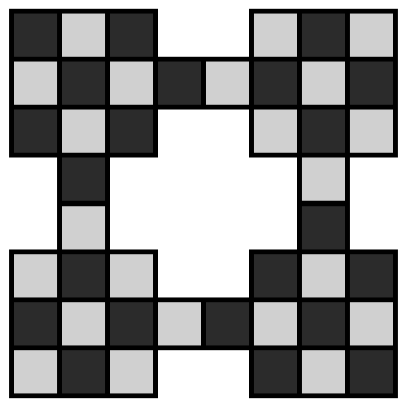
\includegraphics[width=.6\textwidth]{img/ROZ_1_5}
\end{figure}

\section{Rozgrzewka przed kolokwium II}
\paragraph{Zad.1} Złośliwa czarownica wymazała niektóre liczby z poniższego laplasjanu pewnego grafu (znaki ,,?''). Uzupełnij laplasjan i wyznacz liczbę drzew rozpiętych w tym grafie.
$$\begin{bmatrix}
3& ?& -1& -1\\
-1& ?& -1& ?\\
-1& ?& ?& -1\\
?& ?& -1& 2
\end{bmatrix}$$

\paragraph{Zad.2} Oto laplasjan $L$ pewnego grafu G, o którym wiadomo, że największej wartości własnej macierzy $L$ odpowiada wektor $(1, 1, 1, 1, 1, 1, -1, -1, -1, -1, -1, -1)$. Oszacuj z góry jak najlepiej potrafisz liczbę krawędzi w największym cięciu grafu $G$.

\begin{figure}[H]
\centering
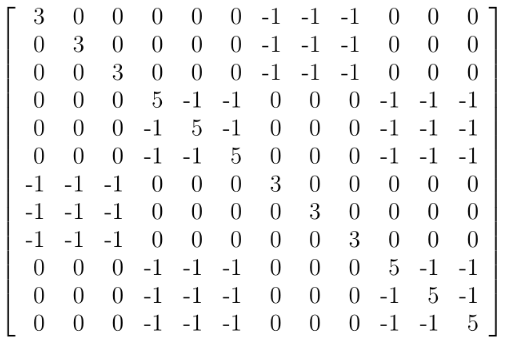
\includegraphics[width=.6\textwidth]{img/ROZ_2_2}
\end{figure}

\paragraph{Zad.3} Znajdź bazę ortonormalna, składającą się z wektorów własnych dla grafu $G$ na sześciu wierzchołkach o dwóch składowych, z których jedna to krawędź izolowana, a druga to $K_4$.

\paragraph{Zad.4} Wyznacz rozkład stacjonarny dla błądzenia po grafie, w którym w każdym kroku z wierzchołka $v$ przechodzimy do każdego z sąsiadów $v$ z prawdopodobieństwem $\sfrac{1}{\deg  (v)^2}$, a pozostajemy w miejscu z prawdopodobieństwem $1 - \sfrac{1}{\deg (v)}$. Fakt, że znaleziony przez Państwa rozkład jest stacjonarny, należy oczywiście uzasadnić.

\paragraph{Zad.5} Zaproponuj prosty algorytm, generujący za pomocą łańcucha Markowa las w grafie $G$ w taki sposób, że po wielu krokach otrzymamy w przybliżeniu każdy las $L$ z prawdopodobieństwem proporcjonalnym do $4^{|E(L)|}$. Poprawność algorytmu należy uzasadnić.

\paragraph{Zad.6} Tasujemy talię 3 kart $A$, $B$ i $C$, w następujący sposób: w każdym kroku wybieramy z jednakowym prawdopodobieństwem kartę środkową lub spodnią i przekładamy ją na wierzch talii. Skonstruuj łańcuch Markowa odpowiadający temu procesowi, wypisz macierz przejścia dla tego łańcucha i sprawdź czy
\begin{enumerate}[label=\alph*)]
\item jest on nieprzywiedlny i nieokresowy?
\item jest odwracalny?
\item posiada rozkład stacjonarny jednostajny?
\item posiada więcej niż jeden rozkład stacjonarny?
\end{enumerate}

\section{Rozgrzewka przed kolokwium III}
\paragraph{Zadanie 1} Skonstruuj odpowiednie sprzęgnięcie (coupling) pokazujące, że powolne błądzenie po $K_{n,n}$ szybko się miesza (tzn. należy oszacować z góry czas mieszania $\tau$ ). Przypominamy, że przy błądzeniu powolnym pozostajemy w wierzchołku $v$ z prawdopodobieństwem $\sfrac{1}{2}$, a przechodzimy do sąsiada $v$ z prawdopodobieństwem $\sfrac{1}{2\deg (v)}$.

\paragraph{Zadanie 2} Tasujemy talię $n$ różnych kart w następujący sposób : zaczynamy od dowolnego stosu, wybieramy losowo (z jednakowym prawdopodobieństwem) jedną z $n$ kart i kładziemy ją na wierzch. Chcemy uzasadnić, że odpowiadający takiemu tasowaniu łańcuch Markowa szybko się miesza i w tym celu definiujemy następujące sprzęgnięcie : Zaczynamy od dwóch różnych permutacji (stosów) naszej talii. W każdym kroku wybieramy losowo w sposób jednostajny kartę z pierwszego stosu, z drugiego stosu wyciągamy kartę taką samą a następnie w obu stosach wybraną kartę przekładamy na wierzch. Uzasadnij, analizując powyższe sprzęgnięcie, że czas mieszania $\tau$ łańcucha wynosi $O(n \log n)$, tzn. $\tau \leq cn \log n$ dla pewnej stałej $c > 0$.

\paragraph{Zadanie 3} Czy istnieje ciało $Q$, liczba naturalna $n$ i kod liniowy $C \subseteq Q^n$, który jest doskonały, ma rozstęp $3$ i składa się z $16$ wyrazów ($|C| = 16$) ? Jeżeli nie – uzasadnij, dlaczego. Jeżeli tak – podaj przykładową macierz generującą taki kod.

\paragraph{Zadanie 4} Oto macierz generująca pewnego kodu $C$ nad ciałem $\mathtt{Z}_3$ :
$$\begin{bmatrix}
1& 1& 1& 1& 2\\
2& 1& 2& 1& 0
\end{bmatrix}$$

Niech $\bar{y} = 11211 \in \mathtt{Z}^5_3$.
\begin{enumerate}[label=\alph*)]
\item Ile wyrazów z $\mathtt{Z}^5_3$
znajduje się w kuli Hamminga o promieniu $2$ i środku w $\bar{y}$?
\item Wyznacz macierz parzystości kodu $C$ i przy jej pomocy sprawdź, czy $\bar{y} \in C$.
\item Wyznacz wszystkie wyrazy $\bar{e}$ o tym samym indeksie co $\bar{y}$ o najmniejszej wadze (czyli będące w najmniejszej odległości Hamminga od $00000$). Jaka jest najmniejsza liczba współrzędnych, jakie musimy zmienić w $\bar{y}$, aby otrzymać wyraz kodu ?
\item Czy kod $C$ jest doskonały ?
\end{enumerate}

\paragraph{Zadanie 5} Przypuśćmy, że mamy zmaksymalizować funkcję $$f(x, y, z) = 2x - 3y$$ w obszarze, w którym $x + y \leq 23$, $x + y + 2z \leq 12$, $y + z \leq 4$, $3x + z \leq 15$. Zamień ten problem na równoważny problem dualny, dotyczący minimalizacji pewnej funkcji liniowej.

\paragraph{Zadanie 6} Fabryka czekolady produkuje różne smakołyki, podzielone na dwie główne kategorie: z czekolady białej i czekolady deserowej. Szef fabryki ma bazę $m$ klientów, dzięki której wie, jakie produkty kto kiedykolwiek kupił. Postanowił zbadać opinie klientów o $p$ produktach, wysyłając kwestionariusz do każdego z nich. Aby nie zniechęcać klientów do jego wypełnienia, kwestionariusz nie może być za długi. Szef przyjął zatem następujące założenia:
\begin{itemize}
\item nie można pytać o produkt, którego klient nigdy nie kupił;
\item produktów z czekolady białej, o które pytamy $i$– tego klienta, nie może być więcej niż $b_i$ (dla $i = 1, . . . , m$);
\item produktów z czekolady deserowej, o które pytamy $i$– tego klienta, nie może być więcej niż $d_i$ (dla $i = 1, . . . , m$);
\item aby badanie było wiarygodne, każdy produkt $j$ musi być oceniony przez co najmniej $k_j$ klientów.
\end{itemize}

Zakładamy, że dysponujemy tylko algorytmem znajdują cym największy przepływ i najmniejsze cięcie w sieciach z jednym źródłem i jednym ujściem. Jak rozstrzygnąć, czy przygotowanie takich kwestionariuszy jest możliwe? Odpowiedź powinna być dokładnie uzasadniona.


\end{document}

\begin{document}



\end{document}
\begin{document}



\end{document}